\documentclass[10pt]{article}
\usepackage[a4paper,margin=2.2cm]{geometry}
\usepackage{amsmath,amssymb}
\usepackage{graphicx}
\usepackage{booktabs}
\usepackage{xcolor}
\usepackage{listings}
\usepackage[font=small,labelfont=bf]{caption}
\usepackage[colorlinks,linkcolor=blue,urlcolor=blue,citecolor=blue]{hyperref}
\graphicspath{{../../figures/}}

\definecolor{codebg}{RGB}{246,247,249}
\lstset{language=Python, basicstyle=\ttfamily\small, backgroundcolor=\color{codebg},
  keywordstyle=\color{blue!70!black}, commentstyle=\color{gray}, stringstyle=\color{orange!70!black},
  frame=single, rulecolor=\color{gray!30}, columns=fullflexible, keepspaces=true,
  aboveskip=6pt, belowskip=6pt, xleftmargin=4pt, xrightmargin=4pt}

\newcommand{\code}[1]{\texttt{#1}}

\title{\textbf{Implementation Details}\\[2pt]\large PINNs for 1D heat diffusion --- repository \code{pinn-heat-diffusion\_1D}}
\author{Quentin Pontalier}
\date{\today}

\begin{document}
\maketitle
\tableofcontents

\section{Scope}
This document describes, exhaustively, what the code in this repository does: every modelling choice, hyperparameter, random seed and evaluation protocol behind the figures and numbers in the \code{README}. A reader should be able to reimplement the results from this document alone. The scientific background is summarized in the technical note (\code{docs/note}).

\section{Problem and synthetic data}

\subsection{Governing equations}
\begin{equation}
\partial_t T = \alpha\,\partial_{xx}T,\qquad x\in[0,L],\ t\in[0,t_{\max}],\qquad
T(x,0)=\sin(\pi x/L),\quad T(0,t)=T(L,t)=0,
\end{equation}
with $L=1$ and $t_{\max}=1.5$. The exact solution and its sensitivity to $\alpha$ (\code{pinn\_heat/physics.py}) are
\begin{equation}
T(x,t)=\sin(\pi x/L)\,e^{-\alpha k^2 t},\qquad
S_\alpha(x,t)=\frac{\partial T}{\partial\alpha}=-k^2\,t\,T(x,t),\qquad k=\pi/L .
\end{equation}

\subsection{Noisy observations}
\code{data.noisy\_observations(n, alpha, noise\_level, seed)} proceeds as follows:
\begin{enumerate}
\item It creates a NumPy generator \code{np.random.default\_rng(seed)}.
\item It draws $n$ locations independently: $t_i\sim\mathcal{U}(0,t_{\max})$, then $x_i\sim\mathcal{U}(0,L)$.
\item It computes $T_i^{\text{clean}}$ from the exact solution and sets $\sigma=\eta\cdot\mathrm{std}(T^{\text{clean}})$, where $\eta$ is \code{noise\_level} and the standard deviation is taken over the $n$ drawn points.
\item It adds noise: $T_i^{\text{obs}}=T_i^{\text{clean}}+\sigma\,\xi_i$, with $\xi_i\sim\mathcal{N}(0,1)$.
\item It discards every observation with $T_i^{\text{obs}}<0$ (\code{drop\_negative=True}). Such values lie below the noise floor and contradict the physics of this problem. The number of points actually kept is reported (e.g.\ 24 of 25).
\end{enumerate}
The noise level is therefore relative to the \emph{spread} of the clean signal, not to each point's value. The exact solution is used only to generate data and to evaluate errors; it never enters the PINN loss.

\subsection{Collocation points}
The PDE residual is evaluated at $N_f=500$ points drawn by Latin Hypercube Sampling:
\code{scipy.stats.qmc.LatinHypercube(d=2, seed=seed)}, scaled to $[0,t_{\max}]\times[0,L]$. They are drawn once and kept \emph{fixed} throughout training. This is required for L-BFGS, which builds its curvature model on a fixed objective.

\section{Network}

\subsection{Architecture and initialization}
\code{model.init\_mlp(key, width=16, depth=3)} builds a fully connected network with layer sizes $[2,16,16,16,1]$. The input is the raw pair $(t,x)$ in that order, with no normalization. Hidden layers use $\tanh$; the output layer is linear. Each layer is initialized with Glorot-uniform weights and zero biases:
\begin{equation}
W\sim\mathcal{U}\!\left(-\sqrt{6/(n_{\text{in}}+n_{\text{out}})},\ \sqrt{6/(n_{\text{in}}+n_{\text{out}})}\right),\qquad b=0 .
\end{equation}
The PRNG key \code{jax.random.PRNGKey(seed)} is split into one sub-key per layer. The network has 609 trainable weights and biases.

\subsection{Hard-constrained ansatz}
The temperature is not the raw network output:
\begin{equation}
T_\theta(x,t)=\sin(\pi x/L)+t\,x\,(L-x)\,\mathcal{N}_\theta(t,x).
\end{equation}
The prefactor $t\,x\,(L-x)$ vanishes at $t=0$, $x=0$ and $x=L$. The initial and both boundary conditions therefore hold exactly for any weights, and no IC/BC loss terms are needed.
\begin{lstlisting}
def temperature(layers, t, x, L=1.0):
    n = mlp(layers, jnp.stack([t, x]))[0]
    return jnp.sin(jnp.pi * x / L) + t * x * (L - x) * n
\end{lstlisting}

\subsection{Diffusivity parameterization (inverse problem)}
The trainable variable is $\beta$, with $\alpha=\alpha_{\min}+\beta^2$ and $\alpha_{\min}=10^{-12}$. This guarantees $\alpha>0$ throughout training. It is initialized at $\beta_0=\sqrt{\alpha_0-\alpha_{\min}}$, with $\alpha_0=1.0$ by default. In the forward problem $\alpha$ is a fixed constant and only the network is trained.

\section{Loss}

\subsection{PDE residual}
The residual is computed pointwise by automatic differentiation and vectorized over the collocation points with \code{jax.vmap}:
\begin{lstlisting}
def pde_residual(layers, alpha, t, x, L=1.0):
    T_t  = jax.grad(temperature, argnums=1)(layers, t, x, L)
    T_xx = jax.grad(jax.grad(temperature, argnums=2), argnums=2)(layers, t, x, L)
    return T_t - alpha * T_xx
\end{lstlisting}
The derivatives are exact, with no finite differences, and they are taken through the full ansatz, including the $\sin$ term and the prefactor.

\subsection{Total loss}
\begin{equation}
\mathcal{L}(\theta,\beta)=\underbrace{\frac{1}{N_f}\sum_{j=1}^{N_f}R(x_j,t_j)^2}_{\mathcal{L}_{\text{phys}}}
\;+\;\lambda\,\underbrace{\frac{\sum_{i=1}^{N_d}w_i\,\big(T_\theta(x_i,t_i)-T_i^{\text{obs}}\big)^2}{\sum_{i=1}^{N_d}w_i}}_{\mathcal{L}_{\text{data}}} ,
\end{equation}
with $\lambda=1$. The weights default to $w_i=1$, in which case $\mathcal{L}_{\text{data}}$ is the ordinary MSE. The forward problem uses $\mathcal{L}_{\text{phys}}$ only. Dividing by $\sum w_i$ keeps the scale of $\mathcal{L}_{\text{data}}$ independent of the weighting law.

\section{Optimization}
Training uses \code{jaxopt.LBFGS} with the settings below. There is no Adam warm-up: L-BFGS starts directly from the initialized weights.
\begin{center}
\begin{tabular}{ll}
\toprule
Setting & Value\\
\midrule
\code{maxiter} & 3000\\
\code{tol} (gradient-norm stopping criterion) & $10^{-9}$\\
\code{history\_size} & 10\\
\code{linesearch} & \code{"zoom"} (strong Wolfe conditions)\\
Precision & float64 (\code{jax\_enable\_x64=True})\\
\bottomrule
\end{tabular}
\end{center}
The loop is written explicitly so that the history can be recorded:
\begin{lstlisting}
state = solver.init_state(params)
update = jax.jit(solver.update)
for it in range(maxiter):
    params, state = update(params, state)
    history["loss"].append(float(state.value))
    history["alpha"].append(float(get_alpha(params)))
    if not np.isfinite(history["loss"][-1]) or float(state.error) < tol:
        break
\end{lstlisting}
Training stops when the gradient norm falls below \code{tol}, when the loss becomes non-finite, or at \code{maxiter}. The forward run reported below used all 3000 iterations. There are no other early-stopping criteria.

Double precision matters: with float32, the second derivatives and the small late-time temperatures ($T\sim10^{-2}$ to $10^{-3}$) lose several significant digits.

\section{Sensitivity-weighted inverse training}
\code{inverse.fit\_inverse\_two\_stage} works in two stages:
\begin{enumerate}
\item \textbf{Stage 1.} A standard inverse fit with $w_i=1$ gives $\alpha_1$.
\item \textbf{Weights.} For each observation,
\begin{equation}
w_i=\max\!\left(\left(\frac{|S_\alpha(x_i,t_i;\alpha_1)|}{\max_k|S_\alpha(x_k,t_k;\alpha_1)|}\right)^{p},\ w_{\min}\right),\qquad p=\tfrac12,\ w_{\min}=0.05 .
\end{equation}
The exponent $p=1/2$ softens the concentration around the sensitivity peak; $w_{\min}$ keeps weakly informative points in the loss. The weights are then frozen.
\item \textbf{Stage 2.} A new fit from scratch, with the same initialization seed, collocation points and $\alpha_0$, using these weights in $\mathcal{L}_{\text{data}}$. The result $\alpha_2$ is the reported estimate.
\end{enumerate}
The weights enter the data term only. The PDE residual must hold everywhere, including in regions that carry little information about $\alpha$. Weighting the IC/BC would be meaningless here anyway, since they are imposed exactly.

\paragraph{Important caveat.} $S_\alpha$ is evaluated with its \emph{analytical} formula, taken at the PINN estimate $\alpha_1$ and never at the true $\alpha$. In a real problem the analytical formula is unavailable. $S_\alpha$ would then have to be estimated from the PINN itself, for example by finite differences between PINNs trained at $\alpha_1\pm\delta$, or by solving the sensitivity equation $\partial_t S=\alpha\,\partial_{xx}S+\partial_{xx}T$.

\section{Evaluation and figures}
\begin{itemize}
\item \textbf{Forward error.} The prediction is evaluated on a uniform $200\times200$ grid over $[0,t_{\max}]\times[0,L]$. The script reports the relative error $\|T_\theta-T\|_2/\|T\|_2$ and the maximum absolute error.
\item \textbf{Inverse error.} The script reports $|\hat\alpha-\alpha|/\alpha$, where $\hat\alpha$ is the value after the last iteration.
\item \textbf{Animations.} A callback records $T_\theta(x,t_k)$ on 120 points in $x$, at $t_k\in\{0,0.15,0.4,0.8,1.5\}$. It does so at 60 log-spaced iterations (\code{np.geomspace(1, maxiter, 60)}), plus the first and last iterations. Log spacing is used because L-BFGS changes the solution mostly in the first tens of iterations. The GIFs play at 10 fps and hold the final frame for 20 frames. In the inverse animation the observations are coloured by their time $t_i$ but plotted against $x$ only, so they do not lie exactly on the displayed profiles.
\end{itemize}

\section{Results}

\subsection{Forward problem}
For $\alpha=0.18$ with seed 0 and 3000 iterations, the final physics loss is $1.38\times10^{-7}$. The relative $L^2$ error is $6.34\times10^{-5}$ and the maximum absolute error $6.17\times10^{-5}$. The run takes 33\,s on a laptop CPU when nothing else is running.

\begin{figure}[h]
\centering
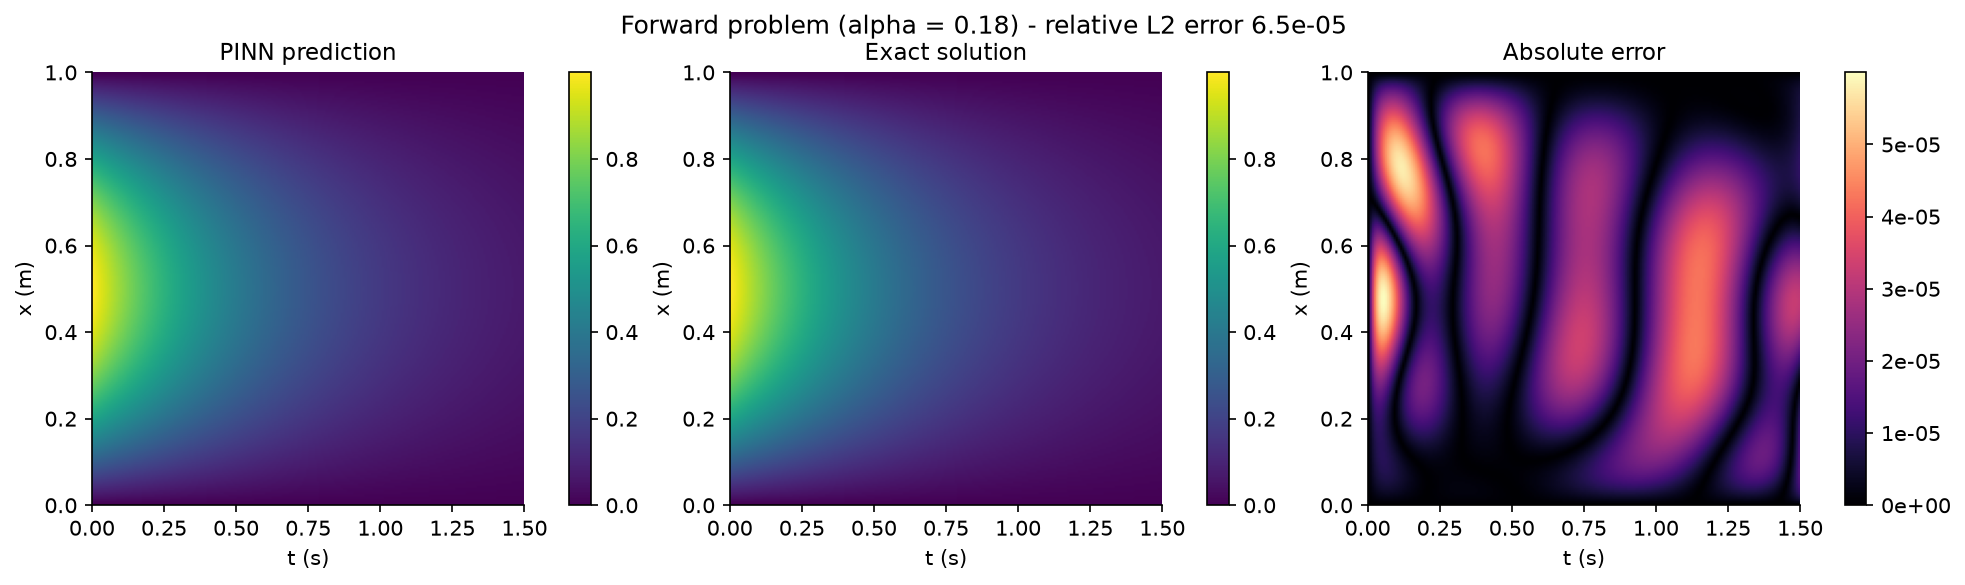
\includegraphics[width=\linewidth]{forward_field.png}
\caption{Forward problem, \code{python scripts/forward.py}.}
\end{figure}

\subsection{Inverse problem, single run}
Settings: $\alpha=0.18$, 25 points drawn, 24 kept, $\eta=10\%$, data seed 0, $\alpha_0=1.0$. The unweighted fit gives $\hat\alpha=0.17800$ (1.11\% error). The two-stage sensitivity-weighted fit gives $\hat\alpha=0.17881$ (0.66\% error).

\begin{figure}[h]
\centering
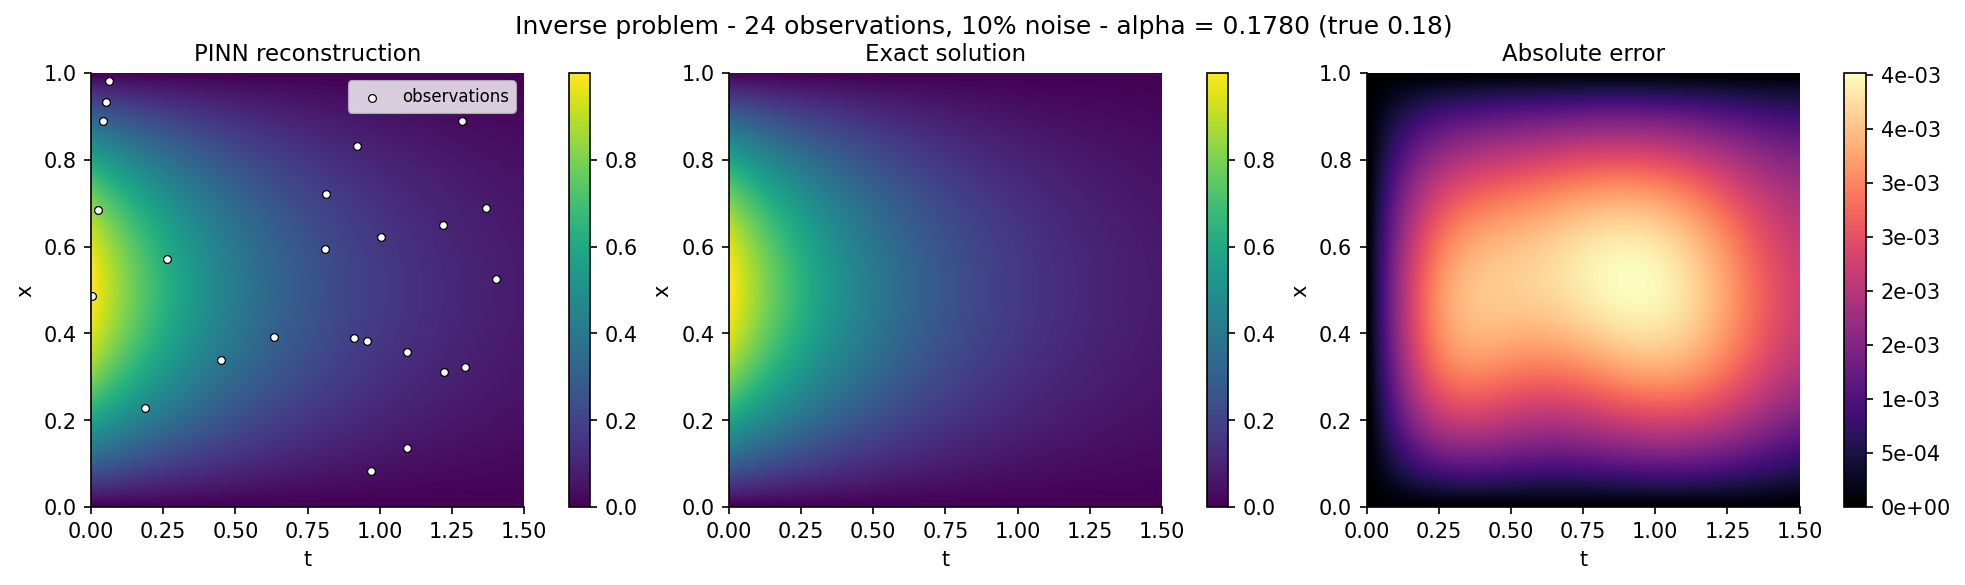
\includegraphics[width=\linewidth]{inverse_field_none.png}
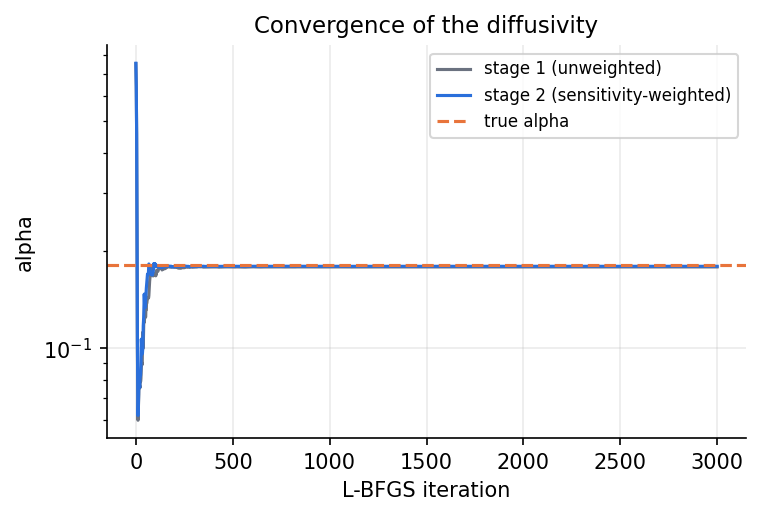
\includegraphics[width=0.55\linewidth]{inverse_alpha_sensitivity.png}
\caption{Top: unweighted inverse reconstruction (\code{python scripts/inverse.py}). Bottom: evolution of $\alpha$ during the two stages (\code{--weighting sensitivity}).}
\end{figure}

\subsection{Robustness study}
\textbf{Protocol} (\code{scripts/robustness\_study.py}):
\begin{itemize}
\item $\alpha\in\{0.18,0.5\}$, $\eta\in\{5,10,20\}\%$ and data seeds $\{0,1,2\}$, with $N_d=25$ drawn points and $\alpha_0=1.0$.
\item Each dataset is solved unweighted and with the two-stage weighting, which gives 36 results and 54 L-BFGS trainings in total.
\item The network initialization seed and the collocation seed are both fixed at 0 for every run. The spread in the results therefore comes \emph{only} from the data (sampling locations and noise realization), not from the optimization.
\end{itemize}

\begin{table}[h]
\centering
\begin{tabular}{cccc}
\toprule
$\alpha_{\text{true}}$ & noise & unweighted & sensitivity-weighted\\
\midrule
0.18 & 5\% & 0.47 (0.62) & 0.49 (0.88) \\
0.18 & 10\% & 0.94 (1.23) & 0.98 (1.76) \\
0.18 & 20\% & 2.31 (2.76) & 2.26 (3.63) \\
0.5 & 5\% & 0.73 (1.01) & 0.48 (0.59) \\
0.5 & 10\% & 2.35 (4.81) & 1.56 (2.93) \\
0.5 & 20\% & 5.05 (10.02) & 3.34 (6.20) \\
\bottomrule
\end{tabular}
\caption{Relative error on $\hat\alpha$ (\%): mean (max) over 3 datasets of 25 points, $\alpha_0=1.0$.}
\label{tab:robust}
\end{table}

\paragraph{Discussion.} Three observations stand out.
\begin{itemize}
\item \textbf{Accuracy.} $\alpha$ is recovered within $0.5\%$ at $5\%$ noise and within a few percent at $20\%$ noise, starting from a guess that is 2 to 6 times too large. The error grows with the noise level and varies noticeably between datasets.
\item \textbf{Effect of the weighting.} It depends on the regime. For $\alpha=0.18$ it changes nothing measurable (mean errors within $0.05$ percentage points). For $\alpha=0.5$ it reduces the mean error by about one third at every noise level, and the worst case at $20\%$ noise from $10.0\%$ to $6.2\%$. This matches the sensitivity analysis: faster diffusion shrinks the window $t\sim t^\ast=1/(\alpha\pi^2)$ in which measurements are informative, so down-weighting uninformative points matters more.
\item \textbf{Systematic bias.} In all 36 cases $\alpha$ is \emph{underestimated}. A likely cause is the removal of negative measurements. At late times the true temperature is close to zero, so the discarded points are preferentially those with negative noise. The retained late-time data are therefore biased upward, which mimics slower decay, i.e.\ a smaller $\alpha$. Testing this would require repeating the study without the filtering.
\end{itemize}

\section{Reproducibility}
\begin{center}
\begin{tabular}{ll}
\toprule
Software & Version used\\
\midrule
Python & 3.11.14\\
JAX / jaxlib & 0.9.2\\
jaxopt & 0.8.5\\
NumPy & 2.4.3\\
SciPy & 1.17.0\\
pandas & 3.0.0\\
Matplotlib & 3.10.8\\
\bottomrule
\end{tabular}
\end{center}
All runs were performed on CPU. Every source of randomness is seeded: the network initialization (JAX key), the collocation points (LHS seed) and the dataset (NumPy generator). Rerunning a script on the same software stack reproduces the numbers above. Small differences can appear with other versions or hardware because of floating-point reduction order.

\section{Differences from the original research code}
The repository is a condensed rewrite of a larger set of exploratory scripts. The method is the same: hard IC/BC ansatz, $\tanh$ network, Glorot initialization, float64, L-BFGS (\code{jaxopt}, zoom line search, history 10), LHS collocation, $\alpha=\alpha_{\min}+\beta^2$, removal of negative observations, and square-root sensitivity weighting. The deliberate differences are:
\begin{itemize}
\item \textbf{Sensitivity weights.} The original weighting study evaluated $S_\alpha$ at $\alpha_{\text{fit}}$, a least-squares fit of the \emph{exact solution} to the data. This rewrite evaluates it at the PINN's own stage-1 estimate, which is closer to a realistic workflow. A minimum weight $w_{\min}$ is also added.
\item \textbf{Data weight $\lambda$.} Here $\lambda=1$. The original study used the empirical law $\lambda=0.8\,(0.1/\eta)^3$, which depends on the noise level.
\item \textbf{Random number generation.} Datasets use \code{np.random.default\_rng} instead of \code{np.random.seed}, and network layers use split keys instead of the fixed per-layer seeds $100+k$. The sampled points and initial weights therefore differ from those of the original study, and its numbers are not directly comparable.
\item \textbf{Not included.} Early stopping based on MSE thresholds; soft-constraint and normalized formulations; Galerkin-type constraints; local noise estimation; the TensorFlow and PyTorch versions.
\end{itemize}

\section{Known limitations}
\begin{itemize}
\item The sensitivity used for weighting relies on the analytical expression of $S_\alpha$ (see above).
\item $\lambda$, the architecture and the number of collocation points were not tuned in this rewrite.
\item Robustness is assessed over datasets only; a single network and collocation seed is used.
\item The results are for a linear 1D problem with a single-mode analytical solution. They do not by themselves transfer to nonlinear or multi-dimensional problems.
\item \code{jaxopt} is no longer actively developed; the L-BFGS implementation in \code{optax} is a natural replacement.
\end{itemize}

\end{document}
